%template1.tex
%The following LaTeX source file represents the simplest kind of slide presentation; no overlays, no included graphics. Substitute your favorite style for ``pascal''. To create the PDF file template1.pdf, (1) be sure to use the prosper class, then (2) execute the command latex template1.tex, and (3) the command dvipdf template1.dvi.

%%%%%%%%%%%%%%%%%%%%%%%%%%%%%%% template1.tex %%%%%%%%%%%%%%%%%%%%%%%%%%%%%%%%%%%
\documentclass[a4paper,blends,pdf,colorBG,slideColor]{prosper}
% definitions for slides for CSC544
% Lutz Hamel, (c) 2007

\hypersetup{pdfpagemode=FullScreen}

\usepackage{times}
\usepackage{latexsym}
\usepackage{alltt}
\usepackage{booktabs}
\usepackage{amsmath}
\usepackage{amsopn}
\usepackage{amsfonts}
\usepackage{amssymb}
%\usepackage[usenames]{color}

\def\sign{\qopname\relax{no}{sign}}
\def\argmax{\qopname\relax{no}{argmax}}
\def\argmin{\qopname\relax{no}{argmin}}

\newcommand{\grad}{\ensuremath{\nabla}} 
\newcommand{\loss}{\ensuremath{{\cal L}}}
\newcommand{\err}{\mbox{err}}
\newcommand{\mse}{\mbox{mse}}
\newcommand{\acc}{\mbox{acc}}
\newcommand{\Integer}{\ensuremath{\mathbb{N}}}
\newcommand{\size}[1]{{|{#1}|}}
\newcommand{\Rnspace}[1]{\ensuremath{\mathbb{R}^{#1}}}
\newcommand{\Real}{\ensuremath{\mathbb{R}}}
\newcommand{\mytt}[1]{{\small\tt{#1}}}
\newcommand{\textemph}[1]{{\em #1}}
\newcommand{\suchthat}{\mid}
\newcommand{\orbar}{\;|\;}
\newcommand{\bs}[1]{\begin{slide}{#1}\ptsize{8}}
\newcommand{\es}{\end{slide}}
\newcommand{\co}{\,\colon\;}
\newcommand{\pair}[2]{\ensuremath{( {#1}, {#2} )}}
\newcommand{\model}[1]{\hat{#1}}
\newcommand{\ul}[1]{{\bf\em #1}}
\newcommand{\ol}{\overline}
\newcommand{\definition}[1]{{\bf Definition: }{\em #1}}
\newcommand{\example}[1]{{\bf Example: }{#1}}
\newcommand{\abs}[1]{|{#1}|}
\newcommand{\mytab}{\makebox[.1in]{}}

\newcommand{\fdef}[1]{
\begin{center}
\fbox{
\begin{minipage}{3.5in}
{\bf Definition:}
{#1}
\end{minipage}
}
\end{center}
}

\newcommand{\fframe}[1]{
\begin{center}
\fbox{
\begin{minipage}{3.5in}
{#1}
\end{minipage}
}
\end{center}
}

\newcommand{\nframe}[1]{
\begin{center}
\begin{minipage}{3.5in}
{#1}
\end{minipage}
\end{center}
}

\newenvironment{Rcode}
	{
		\scriptsize
		\begin{quote}
		\begin{alltt}
	}
	{
		\end{alltt}
		\end{quote}
	}




\begin{document}

\bs{Performance Metrics}
\vspace{.2in}
The simplest performance metric is the {\em model error} defined as the number of mistakes the model makes on a data set divided by the number of observations in the data set,
\begin{equation*}
\err = \frac{\text{number of mistakes}}{\text{total number of observations}}.
\end{equation*}
\es


\bs{The Model Error}
\small
In order to define the model error formally  we introduce the \textemph{0-1 loss function}.  
This function compares the output of a model for a particular observation with the label of this observation.
If the model commits a prediction error on this observation then the loss function returns a 1, otherwise it
returns a 0.

Formally, let  $(\ol{x},y)\in D$ be an observation where
$D \subseteq \Rnspace{n} \times \{+1,-1\}$ 
and let $\model{f}\co \Rnspace{n} \rightarrow \{+1,-1\}$ be a model, then we define the
0-1 loss function $\loss\co \{+1,-1\}\times \{+1,-1\} \rightarrow \{0,1\}$ as,
\begin{equation*}
\loss\left (y,\model{f}(\ol{x})\right ) = \left\{
	\begin{aligned}
	0 & \text{ if $y = \model{f}(\ol{x})$},\\
	1 & \text{ if $y \neq \model{f}(\ol{x})$}.
	\end{aligned}
\right.
\end{equation*}

Let $D = \{(\ol{x}_1,y_1),\ldots,(\ol{x}_l,y_l)\} \subset \Rnspace{n}\times \{+1,-1\}$, 
let the model $\model{f}$ and the loss function $\loss$ be as defined above, then we can
write the model error as,
\begin{equation*}
\err_D[\model{f}] = \frac{1}{l}\sum_{i=1}^{l}\loss\left(y_i, \model{f}(\ol{x}_i)\right ),
\end{equation*}
where $(\ol{x}_i,y_i)\in D$. 

\begin{center}
\fbox{The model error is the {\em average loss} of a model over a data set.}
\end{center}
\es

\bs{Model Accuracy}
\small
We can also characterize the performance of a model in terms of its {\em accuracy},
\begin{equation*}
\acc = \frac{\text{number of correct predictions}}{\text{total number of observations}}.
\end{equation*}
Again, we can use the 0-1 loss function to define this metric more concisely,
\begin{align*}
\acc_D[\model{f}] &= \frac{1}{l}\left(l - \sum_{i=1}^{l}\loss\left (y_i, \model{f}(\ol{x}_i) \right )\right )\\
	&= 1 - \frac{1}{l}\sum_{i=1}^{l}\loss\left (y_i, \model{f}(\ol{x}_i)\right )\\
	&= 1 - \err_D[\model{f}].
\end{align*}
\vspace{.2in}
\begin{equation*}
\boxed{\acc_D[\model{f}]  = 1 - \err_D[\model{f}]}
\end{equation*}
\es

\bs{Example}
As an example of the above metrics, consider a model $\model{g}$ which commits $5$ prediction errors when applied to
a data set $Q$ of length $100$.  We can compute the error as,
\begin{equation*}
\err_Q[\model{g}] = \frac{1}{100}(5) = 0.05.
\end{equation*}
We can compute the accuracy of the model as,
\begin{equation*}
\acc_Q[\model{g}] = 1 - \err_Q[\model{g}] = 1 - 0.05 = 0.95.
\end{equation*}
\es

\bs{Model Errors}
Let $(\ol{x}, y) \in \Rnspace{n}\times\{+1,-1\}$ be an observation and let $\model{f}\co \Rnspace{n} \rightarrow\{+1,-1\}$ be a model, then
we have the following four possibilities when the model is applied to the observation,
\begin{equation*}
\model{f}(\ol{x}) = \left \{
	\begin{aligned}
	+1 & \text{ if $y = +1$, called the {\em true positive}}\\
	-1 & \text{ if $y = +1$, called the {\em\color{red} false negative}}\\
	+1 & \text{ if $y = -1$, called the {\em\color{red} false positive}}\\
	-1 & \text{ if $y = -1$, called the {\em true negative}}\\
	\end{aligned}
\right .
\end{equation*}
This means that models can commit two types of model errors.

Under certain circumstances it is important to distinguish these types of errors when evaluating a
model.

We use a {\em confusion matrix} to report these errors in an effective manner.

\es

\bs{The Confusion Matrix}
\small
A confusion matrix for a binary classification model is a $2\times2$ table that displays the observed labels against the 
predicted labels of a data set.  

\begin{center}
\scriptsize
   \begin{tabular}{ccc}
      \toprule
  Observed ($y$) $\backslash$ Predicted ($\model{y}$) & +1 & -1 \\
     \midrule
      +1      & True Positive (TP) & False Negative (FN)  \\
      -1 & False Positive (FP) & True Negative  (TN) \\
      \bottomrule
   \end{tabular}
\end{center}
   
One way to visualize the confusion matrix is to consider that applying a model $\model{f}$ to an observation $(\ol{x},y)$ will 
give us two labels.  The first label $y$ is  due to the observation and the second label
$\model{y} = \model{f}(\ol{x})$ is due to the prediction of the model.
Therefore, an observation with the label pair $(y,\model{y})$ will be mapped onto 
a confusion matrix as follows,
\begin{center}
\begin{tabular}{ccc}
(+1,+1) & $\mapsto$ & TP\\
(-1,+1) & $\mapsto$ & FP\\
(+1,-1) & $\mapsto$ & FN\\
(-1,-1) & $\mapsto$ & TN
\end{tabular}
\end{center}

\es

\bs{The Confusion Matrix}
{\bf Example:}
\begin{center}
\scriptsize
   \begin{tabular}{ccc}
      \toprule
  Observed $\backslash$  Predicted & +1 & -1 \\
      \midrule
      +1      & 95 & 7  \\
      -1 & 4 & 94\\
      \bottomrule
   \end{tabular}
\end{center}
A confusion matrix of a model applied to 
a set of $200$ observations.  On this set of observations the model commits $7$ false negative errors
and $4$ false positive errors in addition to the $95$ true positive and $94$ true negative
predictions.  
\es

\bs{Example}
Wisconsin Breast Cancer Dataset:

\begin{Rcode}
> library(e1071)
> wdbc.df <- read.csv("wdbc.csv")
> svm.model <- svm(Diagnosis ~ ., 
                   data=wdbc.df, 
                   type="C-classification",
                   kernel="linear", 
                   cost=1)
> predict <- fitted(svm.model)
> cm <- table(wdbc.df$Diagnosis,predict)
> cm
   predict
      B   M
  B 355   2
  M   5 207
> err <- (cm[1,2] + cm[2,1])/length(predict) * 100
> err
[1] 1.230228
\end{Rcode}
\es

\bs{Model Evaluation}
Model evaluation is the process of finding an optimal model for the problem at hand.

You guessed it, we are talking about optimization!

Let,
\begin{equation*}
D = \{(\ol{x}_1,y_1),\ldots,(\ol{x}_l,y_l)\} \subset \Rnspace{n}\times \{+1,-1\}
\end{equation*}
be our training data, then we can write our parameterized model as,

\begin{equation*}
\label{eq:param-model}
\model{f}_D[k,\lambda,C](\ol{x}) = \sign \left ( \sum_{i=1}^l \alpha_{C,i} y_i  k[\lambda](\ol{x}_i,\ol{x}) - b\right ),
\end{equation*}
where $(\ol{x}_i,y_i)\in D$.

With this we can write our model error as,
\begin{equation*}
\err_D\left [\model{f}_D[k,\lambda,C]\right] = \frac{1}{l} \sum_{i=1}^l \loss\left (y_i,\model{f}_D[k,\lambda,C](\ol{x}_i)\right),
\end{equation*}
where $(\ol{x}_i, y_i)\in D$.
\es

\bs{Training Error}
\small
The optimal training error is defined as,
\begin{equation*}
\min_{k,\lambda,C} \err_{\color{red}D}\left [\model{f}_{\color{red}D}[k,\lambda,C]\right] = \min_{k,\lambda,C}\frac{1}{l} \sum_{i=1}^l \loss\left (y_i,\model{f}_D[k,\lambda,C](\ol{x}_i)\right).
\end{equation*}
\vspace{.2in}
\begin{center}
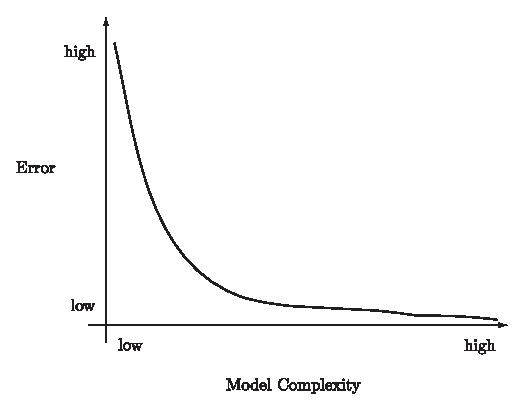
\includegraphics[height=1.8in]{figures/fig09-01.eps}
\end{center}
\es

\bs{Training Error}
{\bf Observation:}

The problem here is that we can always find a set of model parameters that make the 
model complex enough to drive the training error down to zero.

The training error as a model evaluation criterion is overly optimistic.

\es

\bs{The Hold-Out Method}
Here we split the training data $D$ into a {\em training set} and a {\em testing set} 
$P$ and  $Q$, respectively, such that,
\begin{equation*}
D = P \cup Q \text{ and } P\cap Q = \emptyset.
\end{equation*}
The {\em optimal training error} is then computed as
the optimization problem,
\begin{equation*}
\min_{k,\lambda,C} \err_{\color{red}P}\left [\model{f}_{\color{red}P}[k,\lambda,C]\right] = \err_P\left [\model{f}_P[k^{\bullet},\lambda^{\bullet},C^{\bullet}]\right].
\end{equation*}
Here, the optimal training error is obtained with model $\model{f}_P[k^{\bullet},\lambda^{\bullet},C^{\bullet}]$.

The {\em optimal test error} is computed as an optimization using $Q$ as the test set,
\begin{equation*}
\min_{k,\lambda,C} \err_{\color{red}Q}\left [\model{f}_{\color{red}P}[k,\lambda,C]\right] = \err_Q\left [\model{f}_P[k^*,\lambda^*,C^*]\right].
\end{equation*}
The optimal test error is achieved by some model $\model{f}_P[k^*,\lambda^*,C^*]$.

\es


\bs{The Hold-Out Method}
\begin{center}
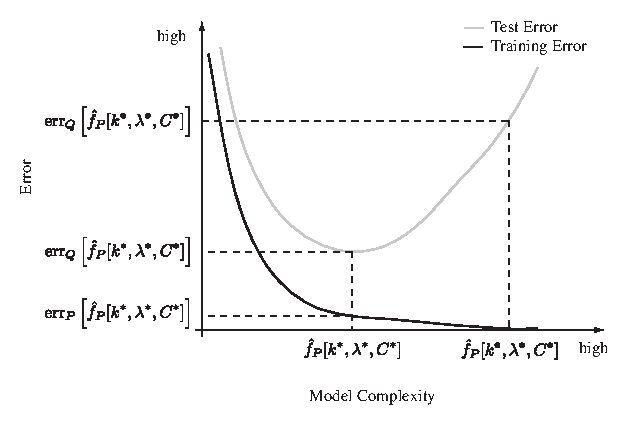
\includegraphics[width=4in]{figures/fig09-02.eps}
\end{center}
\es


\end{document}
%%%%%%%%%%%%%%%%%%%%%%%%%%% end of template1.tex %%%%%%%%%%%%%%%%%%%%%%%%%%%%%%%%

